\subsection{5 GHz}
The data gathered during the 5 GHz measurements proved to be less interesting than the data we gathered in the 2.4 GHz measurements. Most of the channels we measured turned out to be empty or contain very little signal which might have been expected given the number of channels available. For the most part, the channels that did show traffic did not show any significant patterns or recurring phenomena though there are some exceptions. An example such an exception was the cot-node3-student, that showed a lower amount of traffic for some time around noon on both May 17th and May 22nd. The reason for this however is not as apparent as the cause of the pattern in the 2.4 GHz case where we saw an absence of a spike in traffic during the daytime on the schoolnode. It might be that the decrease occurs every couple of days, for example due to a router switching channels temporarily or restarting or the decrease might simply be an anomaly, this would require further investigation. (TODO does this make sense)
\begin{figure}[h!]
    \centering
    \textbf{cot-node3-student, channel 36, 15/05 - 22/05}\par\medskip
	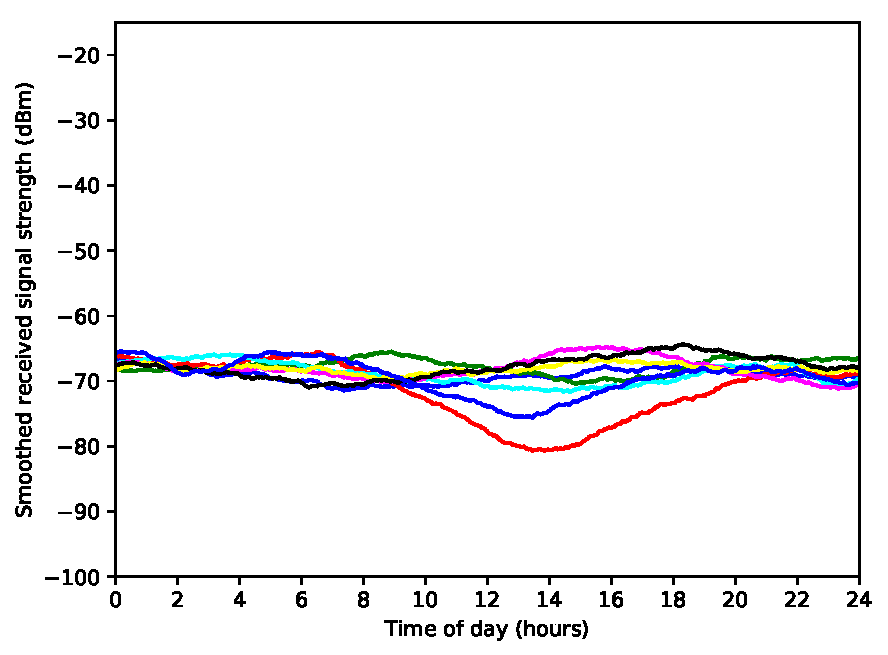
\includegraphics[scale=0.5]{images/5_GHz/cot-node3-student_2017-05-22_chan36_image.pdf}
\end{figure}\\
This graph was generated from our cot-node3-student data discarding the highest 5 (out of roughly 700) signals to combat outliers skewing the graph. The real graph could be a few dBm higher but the result would be no different : the channel is moderately used but there is room for more traffic. On other channels, this node sees barely any traffic in the 5 GHz band. \\
For the 5 GHz band it is worth noting that the measurements we have from our indoor nodes show some difference from those measured by the outdoors node when looking at channels other than channel 36. The outdoor node has at least some traffic on every channel whereas most of the indoors nodes show the bare minimum of traffic for most channels. An example of the outdoors node's traffic on channel 56 versus an indoors node on that same channel is shown below:
\begin{figure}[h!]
    \centering
    \textbf{node1, channel 56, 13/05 - 17/05}\par\medskip
	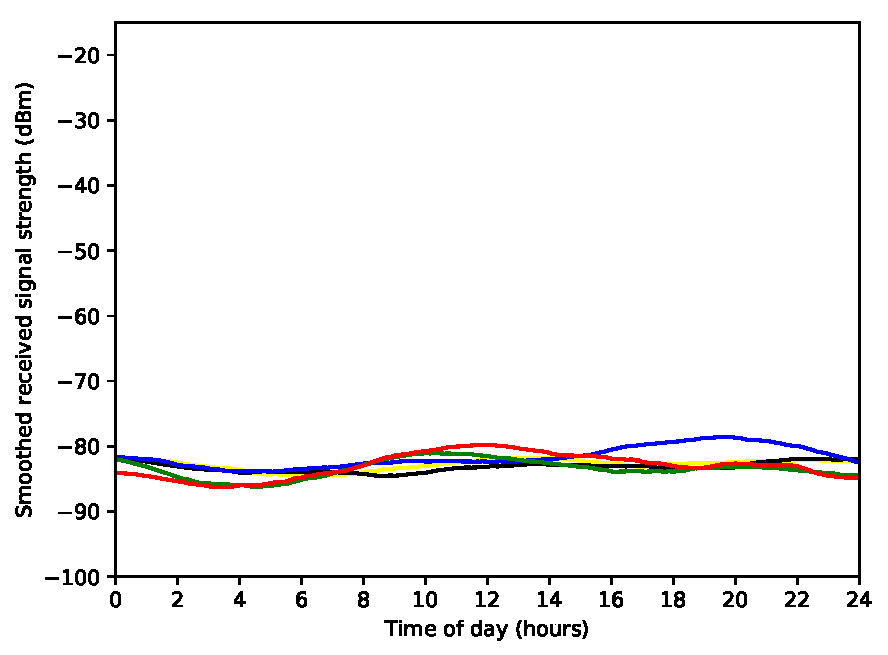
\includegraphics[scale=0.5]{images/5_GHz/node1_2017-05-17_chan56_image.pdf}
\end{figure}\\
\begin{figure}[h!]
    \centering
    \textbf{cot-node3-student, channel 56, 15/05 - 21/05}\par\medskip
	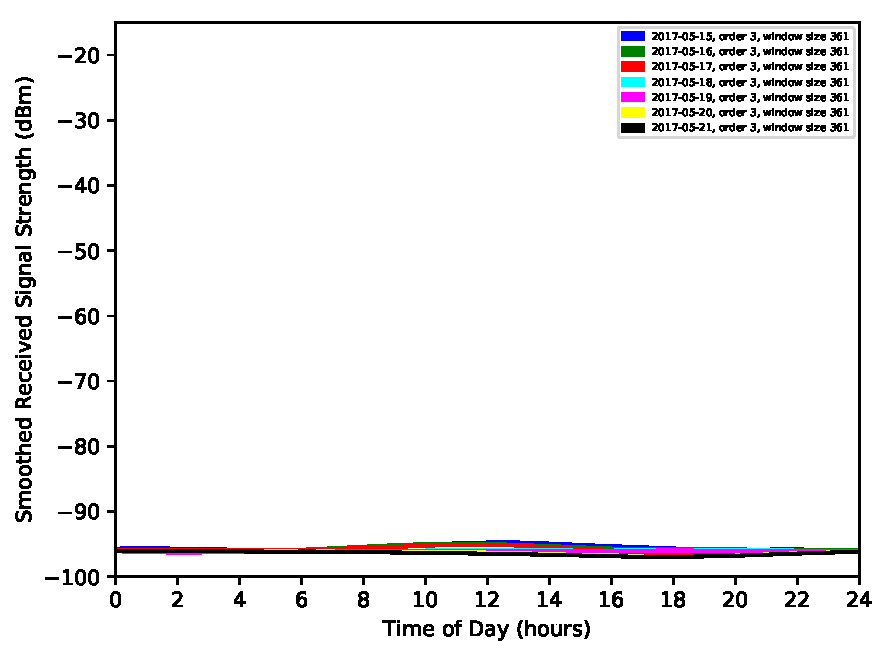
\includegraphics[scale=0.5]{images/5_GHz/cot-node9-student_2017-05-21_chan56_image.pdf}
\end{figure}\\
Which can be attributed to the outdoor node being outdoors and thus having less trouble picking up 5 GHz signals as they penetrate buildings and walls less easily.\\  \\
There were some other interesting phenomena we observed in the 5 GHz channels, for example the following two graphs paired with a decrease of the signal strength on channel 120 for the same node, as shown on the third graph: \newpage
\begin{figure}[h!]
    \centering
    \textbf{cot-node6-student, channel 56, 12/05 - 20/05}\par\medskip
	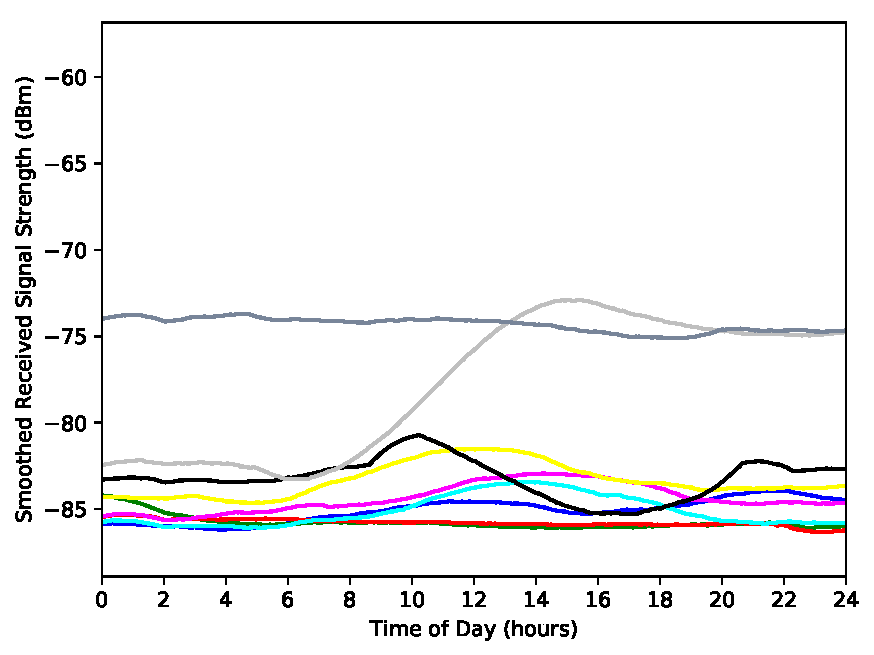
\includegraphics[scale=0.5]{images/5_GHz/cot-node6-student_2017-05-20_chan56_image.pdf}
\end{figure}\\
\begin{figure}[h!]
    \centering
    \textbf{cot-node6-student, channel 64, 12/05 - 20/05}\par\medskip
	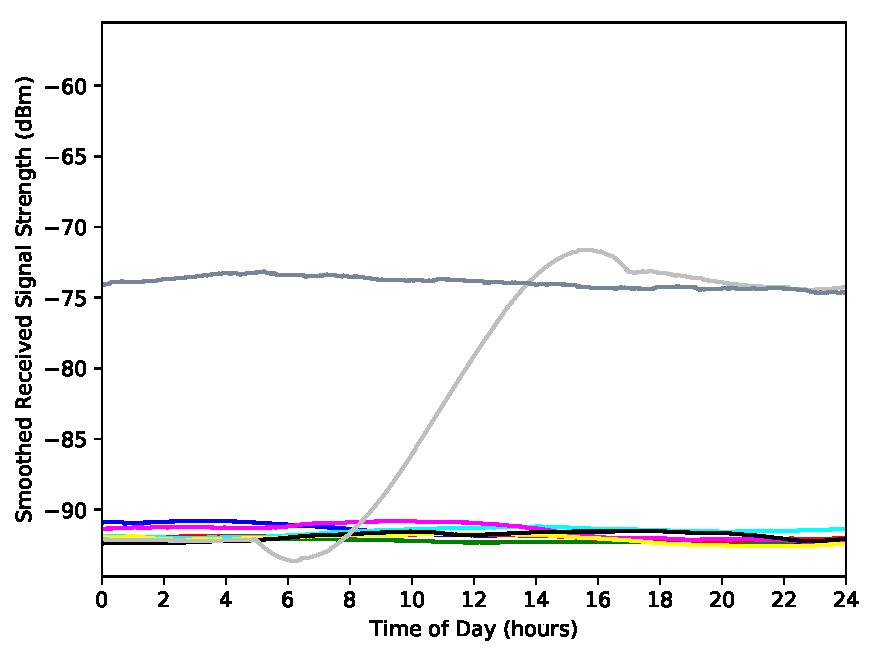
\includegraphics[scale=0.5]{images/5_GHz/cot-node6-student_2017-05-20_chan64_image.pdf}
\end{figure}\\

\begin{figure}[h!]
    \centering
    \textbf{cot-node6-student, channel 120, 12/05 - 20/05}\par\medskip
	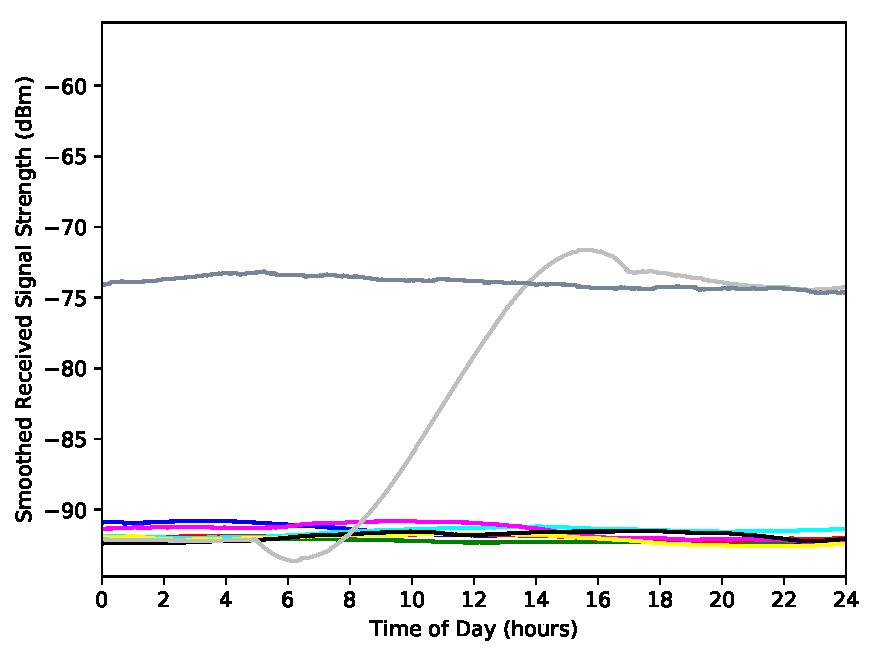
\includegraphics[scale=0.5]{images/5_GHz/cot-node6-student_2017-05-20_chan64_image.pdf}
\end{figure}\\
which seems to show some traffic moving from channel 120 to channel 56 and / or 64 (TODO why doesnt it show on chan60?) on friday May 19th, which lasts all the way through saturday May 20th. We could not confirm when or if the signal ends due to the aforementioned (presumed) hardware failure. This signal still only amounts to an estimated signal strength of about -70 dBm which should still leave enough room for other traffic on the channel and in the spectrum.\\
For some nodes (all but cot-node6-student, cot-node8-student and node1), checking the higher up channels (the channels numbered 100 and above) shows no traffic on any of the nodes for those channels. For the three nodes mentioned, the fact that node1 shows some traffic on these channels is consistent with earlier observations of the outdoor node seeing more traffic on the 5 GHz band than the indoor nodes. For nodes cot-node6-student and cot-node8-student we don't have an explanation for why they have more traffic on these channels than the other nodes. Fact remains that the 100+ channels are relatively empty.
Included below are three graphs for three of our nodes; cot-node3-student, cot-node8-student and node1. Each of these was somewhat busy on the 2.4 GHz band, showed some traffic on the lower 5 GHz channels and demonstrates our findings for the higher channels:
\begin{figure}[h!]
    \centering
    \textbf{cot-node3-student, channel 100, 15/05 - 22/05}\par\medskip
	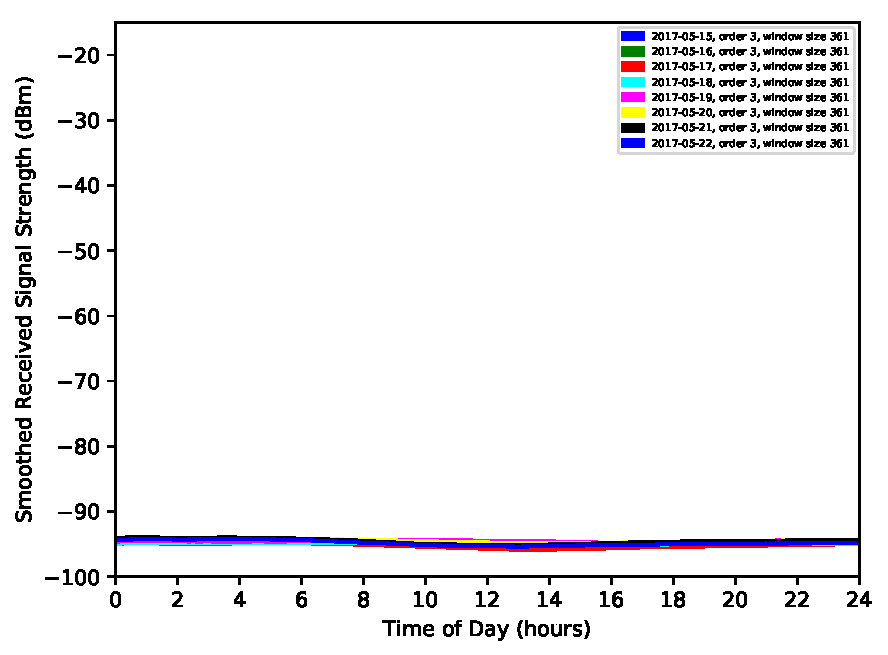
\includegraphics[scale=0.4]{images/5_GHz/cot-node3-student_2017-05-22_chan100_image.pdf}
\end{figure}\\
\begin{figure}[h!]
    \centering
    \textbf{cot-node12-student, channel 120, 12/05 - 16/05}\par\medskip
	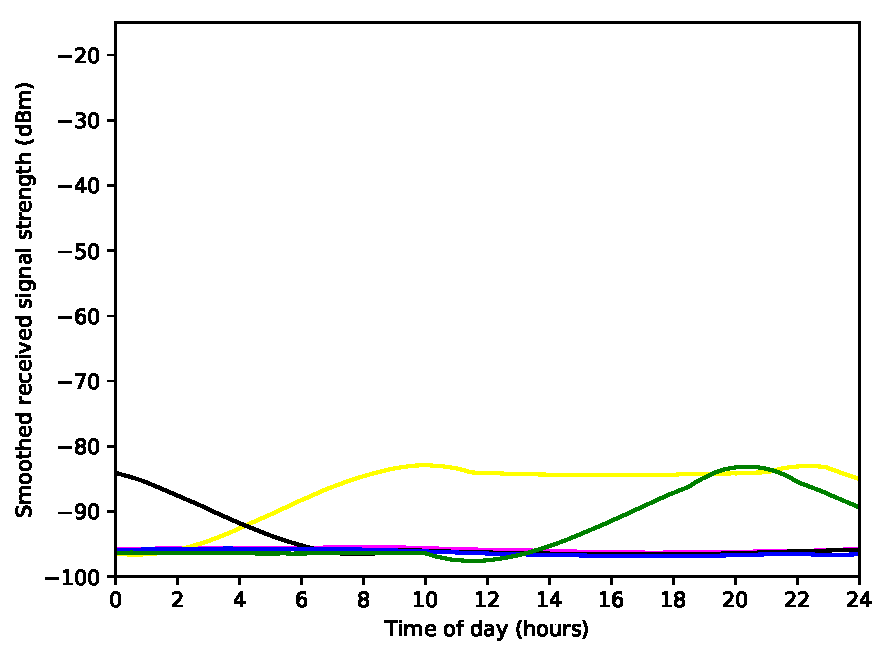
\includegraphics[scale=0.4]{images/5_GHz/cot-node8-student_2017-05-16_chan120_image.pdf}
\end{figure}\\
\begin{figure}[h!]
    \centering
    \textbf{node1, channel 140, 13/05 - 17/05}\par\medskip
	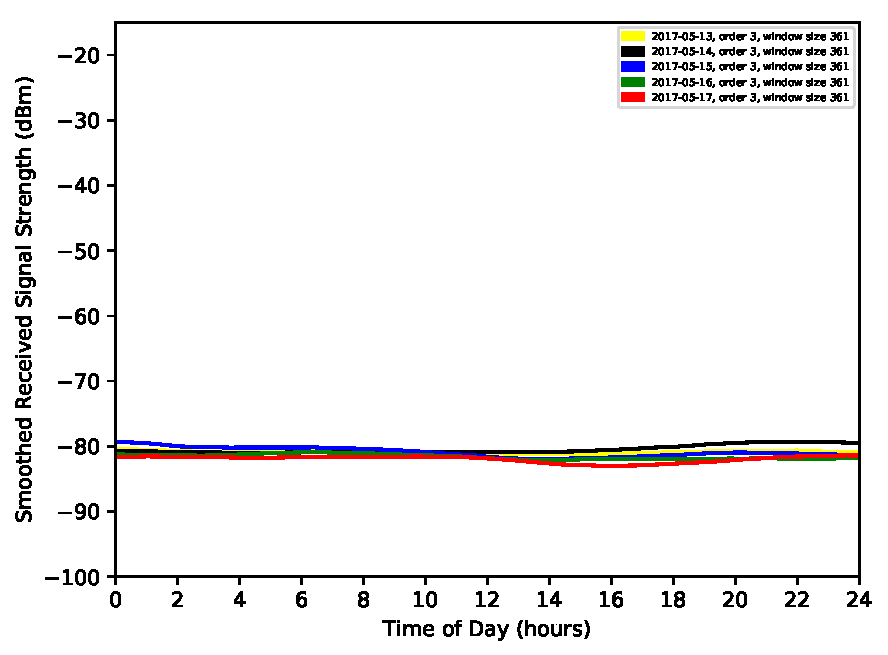
\includegraphics[scale=0.4]{images/5_GHz/node1_2017-05-17_chan140_image.pdf}
\end{figure}\\
